\documentclass[a4paper,11pt]{article}
\usepackage[T1]{fontenc}
\usepackage{inputenc}
\usepackage{amsfonts}
\usepackage{graphicx}
\usepackage{bm}
\usepackage{varioref}
\usepackage[english]{babel}
\usepackage{hyperref}
\usepackage{tikz}
\usetikzlibrary{arrows,decorations.pathmorphing,backgrounds,positioning,fit,petri}
\usepackage{enumitem}
\usepackage{newclude}
\newcommand{\field} [1] {\mathbb{#1}}
\newcommand{\hiddensubsubsection}[1]{
	\stepcounter{subsubsection}
	\subsection*{\Alph{section}.\arabic{subsection}.\arabic{subsubsection}\hspace{1em}{#1}}
}
\begin{document}

\begin{titlepage}
\centering \parindent=0pt
\newcommand{\HRule}{\rule{\textwidth}{1mm}}
\vspace*{\stretch{1}} \HRule\\[1cm]\Huge\bfseries
Roadmap\\[0.7cm]
\large Visualisation and path finding\\[1cm]
\HRule\\[4cm]  \large by \\Jacob Stenum Czepluch (jstc@itu.dk), \\Niels Liljedahl Christensen (nlch@itu.dk), \\Mikkel Larsen (milar@itu.dk), \\Sigurt Bladt Dinesen (sidi@itu.dk) \\
\vspace*{\stretch{2}} \normalsize %
\begin{flushleft}
IT-University\\
Copenhagen\\
First year project\\
Rasmus Pagh\\
\today \end{flushleft}
\end{titlepage}

\tableofcontents
\pagebreak

\pagebreak
\section{Introduction}


\pagebreak
\section{User manual}
An introduction to the application / user manual \ldots

\subsection{Navigating the map}
Explanation of how to navigate the map \ldots

\subsection{Finding specific locations and trips}
Explanation of how to search for locations and trips \ldots

\pagebreak
\section{Design choices}
\label{sec:Design choices}
In this section, we will go through our design choices. We will go through things like design patterns, data structures, and visualisation. At the same time we will gives explanation of our choices.

This section does not contain any information about the implementation of the application, which for several reasons can vary from the design choices made. Variations will be discussed in the Discussion section on page \pageref{sec:Discussion}.

\subsection{Architectural Pattern}
\label{sub:Design Pattern}
For our overall architectural pattern, we have chosen to use the Model, View, Controller (MVC) pattern. We chose to do so, to make sure that we have a very modular and easy-to-maintain class structure. Using the MVC pattern results in separation of the different aspects of our application, while still providing a loose coupling between these elements. During the making of the application it has proven very useful to us since we have been chancing our classes and data structures quite a few times. 

\subsection{Data structures}

\subsubsection{Preprocessed files}
We decided on using preprocessed files containing the edge and vertex data needed to create graphs for path finding, as well as a file for creating our ternary trie and a file containing krak data for each edge (used when drawing roads). Use of the these files speeds up several parts of our application since the files we have to read through contain only the information that is strictly necessary to serve their purposes. Also, since the files only need to be created once (ever), this can be done outside of the application, not adding to the start-up time, and in contrast to having the krak files lying around in the application, these files serve the same purpose but without taking up nearly as much memory.

\subsubsection{The graph}
Our application uses two graphs; one containing edges weighted by time and one containing edges weighted simply by their length. The first of the two is used to compute the fastest path from one given point to another, and the latter of the two is used to compute the shortest path between any two point. 

Each of these graphs consists of an array of vertices, each of which knows its neighbour vertices and edges.		

The shortest path graph could be expanded to allow the choice between different types of transportation (such as walking or cycling) where one is assumed to maintain roughly the same speed throughout the entire trip.

\subsection{Visualisation and user interaction}

\subsubsection{Platform}
To start with we had to decide whether we wanted to use \texttt{Java} and \texttt{Swing}, or \texttt{Java}, \texttt{JavaScript}, \texttt{SVG}, and \texttt{HTML} for the visualisation part. There are strengths and weaknesses to both solutions: The good thing about \texttt{Swing} is that we all have previous experience with it, and so we were certain that, using \texttt{Swing}, we would be able to do what we wanted. 
The fact that none of us have had any notable experience with \texttt{JavaScript} and \texttt{SVG} made it easy for us to decide on a platform for this project. By using \texttt{Java} and \texttt{Swing}, we would be able to spend our time making a well working program with a nice data structure. We would, of course, have liked looking into a new language like \texttt{JavaScript}, but we have chosen to prioritize a well working program over the learning experience of working with a new programming language.

\subsubsection{How the roads are drawn}
As mentioned above we chose to use \texttt{Swing} and the \texttt{BasicStroke API} to do the drawing of the map. 

Technically, the map first draws all of Denmark. It is however only the largest of the road types that is drawn when the whole of Denmark is shown. We decided to only do so because it is both unnecessary to draw all roads when you are very far away from the map, but also to make the program run smoother. The program is designed to show more and more road types the more you zoom in towards the map. Only the roads that are inside the given view are drawn.

We decided to make the thickness of the roads relative (so for example highways are displayed as being wider than smaller roads). The different types of roads are displayed using different colors, making is possible for the user to distinct between them.

\subsubsection{User interaction with the map}
We wanted to make a simple, yet featureful, user interaction with the map. This resulted in a user interface with no physical buttons. All you need to navigate the map is pointing device (i.e., a mouse). To zoom in and out you scroll up and down, respectively. The mouse pointer decides what the zooming point is. It is also very easy to pan up or down, or to the sides. This is done by simply dragging and dropping the map with the mouse pointer. The window is also easily resized by dragging in one corner of the window. There are, however, some differences in the way that the resizing behaves according to the OS the program is running under.

There must be a limit of how far in and out the user can zoom on the map. The limit on zooming out is to avoid the user at some point being zoomed out so far that it is no longer possible to navigate back to display a wished part of the map (and since only the roads of Denmark are to be drawn, nothing will be visible other than maybe a very small amount of pixels representing Denmark). The limit of zooming in must prevent the user from being zoomed in so far the map is no longer recognizable as a map. If no boundaries for zooming were to be made, it is imaginable that the user by accident zooms either too far in or out, no longer recognizing what is displayed. The result is very likely to look similar to no roads being draw at all, which might again cause it to seem as if an error has occurred, forcing the user to restart the application.

Limits must also be present when dragging the current view for similar reasons (Ex. dragging to some places away from the roads drawn, making it look as if no roads are displayed).

We want a user interface design with a minimal number of buttons and other components on the graphical user interface because it, in our strongest conviction, is the most intuitive way for people to navigate and interact with maps. It seems that this has become the \textit{de facto} standard, probably due to the increasing number of tablets and smartphones on the market.

\subsubsection{Finding locations and trips}
As with the user interaction with the map, we decided to make the graphical user interface for finding either a location or a trips as simple as possible (and with that having as few as possible buttons to push and places to type text). The result was having two fields in which addresses can be typed in by the user and a button for executing the search for either location or trip. When the button is pressed, the content of the input fields decides what is to be executed. The possibilities are the following:
\begin{itemize}
	\item \textbf{Only one address is typed in} \\
		A search for the location according to the given address is executed, giving that the address is understood by the application as a valid address.
	\item \textbf{Two addresses are typed in} \\
		A search for the trip from the first given address to the second given address is executing, given both the the addresses are understood by the application as valid addresses.
\end{itemize}
In addition to that, when a search for a trip is executed, the search can actually be of two different types:
\begin{itemize}
	\item A search for the \textit{shortest} trip from one location to another (the one with the shortest distance).
	\item A search for the \textit{fastest} tip from one location to another (the one taking the shortest period of time to follow).
\end{itemize}
This second search criteria is also to be selected by the user. This is to be done with radio buttons allowing the user to toggle between the two.

All input fields, button(s) and radio buttons are to be labeled with either names which in themselves describe the purpose of the component to a satisfactory level, or with a short description of the purpose.

\subsubsection{What is a valid address}
The validity of a typed in address is dependent upon two different things; the \textit{content} of the address and the \textit{format} in which the address is written.

The \textit{content} can be different combinations of the following three:
\begin{itemize}
	\item \textbf{City name} \\
		Containing the letters a - z and A - Z, white spaces, and the letters special the the "Nordic" alphabets.
	\item \textbf{Zip code} \\
		Consisting only of the digits 0 - 9 (without white spaces) and be between 3 and 5 digits long.
	\item \textbf{Street name} \\
		Similar to the city name.
\end{itemize}
It must be possible to search for:
\begin{itemize}
	\item City name only
	\item Zip code only
	\item City name and zip code
	\item Street name with city name and/or zip code
\end{itemize}
This means that in order to find a road, you must include include either the corresponding zip code or city name in the given address.

!!!Maybe move the limitations of the address content Jacob wrote to this place instead?

The \textit{format} must be easy to get used to / similar to the way we write addresses in letters, mails etc.

When writing city name and street name next to each other, they must be separated with one or more characters not "legally" part of either of them. An obvious option is separating the city name and street name with a comma (\texttt{","}) or with a comma followed by a white space (\texttt{", "}), but other characters must be accepted as well.

When writing either city name or street name next to the zip code, it should not be necessary to use any special characters to separate them. For example, it should be possible to write an entire address containing both street name, zip code, and city name without using any special characters to separate them, having the zip code in the middle of the others (Ex. \texttt{"Street name 1234 city"}).

Extra spaces within in in either the beginning or end of a city name or street name should be ignored and not cause the application to not accept the address as being valid (Ex. \texttt{"City    name"}).

It should not matter whether capitalized letters are used or not. Capitalized and non-capitalized letters should be understood as being the same. For example should \texttt{"CiTy NAMe"} and \texttt{"city name"} result in the same address search.

If an address is not accepted as being valid, the user must be alerted, telling which of the addresses which are not valid. A similar such warning must be provided given the user executes a search without having entered any address at all. The user must not be left in a situation where he/she might thinks a search has been executed, though that is not the case.

\subsubsection{Automatic text completion}
In order to aid the user in finding the wanted address with a minimum of clutter and issues with the content and format of the address to be typed in, we want the application to provide the user with a list of the addresses which best match what is currently typed in. The list will be empty when nothing is written, but the content of the list must appear as soon as a characters is typed in, and the list must update for each additional character typed / for each character removed. The list has to contain between zero and five possible addresses.

Why we have decided to display up to five addresses is a matter of taste. We find that it is a reasonable amount of addresses, having enough for the user to have several options to choose between, but not having so many that the list dominates the rest of the graphical user interface.

It has to be possible for the user to select the addresses on the list, copying the selected address to the input field and hiding the list from the view, avoiding that the list is in the way of other operation the user might want to perform.

\subsection{Outline}
\begin{itemize}
	\item Design Pattern \\
		\textsl{Done}
	\item Data structures
	\begin{itemize}
		\item Preprocessed files \\
		We have decided on using preprocessed files containing the edge and vertex data needed to create graphs for pathfinding. This speeds up the graph creation process since the files we have to read through contain only the information that is strictly necessary to create the graphs. Also, since the files only need to be created once (ever), this can be done outside of the application, not adding to the start-up time, and in contrast to having the krak files lying around in the application, these files serve the same purpose but without taking up nearly as much memory.
		\item Storing the edges (quadtrees, in the app and in the file) \\
		\textsl{Niels}
		\item The graph data structures (in the app and the files) \\
		\textsl{Niels}
		\item The Trie data structure (in the app and the files) \\
		\textsl{Sigurt}
	\end{itemize}
	\item Visualisation \\
		\textsl{Mikkel}
	\begin{itemize}
		\item Platform
		\item How the roads are drawn
		\item Finding location
		\item Finding trips
		\item Auto completion
		\item User interaction on the map
	\end{itemize}
	\item Limitations \\
		\textsl{Jacob}
	\begin{itemize}
		\item Not more precise than road names
		    
		    Since it is not required that the program is able to search for road numbers, we decided not to implement them. Another reason to not implement road numbers is that it is not very well defined in the dataset, where a given road number is located on an edge. We would have liked to implement road numbers, but we could not figure out a decent way to do this with the data given from Krak. The biggest and most important consequence of this decision is that on very long roads, it can be very difficult to find a desired exact address, since you will not know in which end or side of the road that the address is located.   

		\item Route description

		    It was part of our plan to make a route description located under the distance and time in the left side of the window. The description should describe when and where to turn and to what side to turn during a trip. It was however a more time consuming implementation than first assumed and we down prioritized the implementation to make sure that we had time to make some of the more important implementations on out list. 

		\item One user, one system

		    Our program is limited to only have one user for each instance of the program. This is due to a couple of things. The main reason is that it never was part of out plan or design decisions to make a multiuser program. Further more would we have to make some quite big changes to out program to make it work with multiple users. Our pathfinding algorithm, is for example, very suitable and acceptable for a singleuser version of the program, but it would be too slow if we had around 100 or more users, because one search using Dijkstra's algorithm takes around 50 or 100 times longer than using the A* algorithm, which we would have to use instead if we were going to make a multiuser version of our program.
	\end{itemize}
\end{itemize}

\pagebreak
\section{Implementation}
\label{sec:Implementation}
The implementation of the application consists of four different packages; the \texttt{Model}, \texttt{View} and \texttt{Controller} packages used as in the MVC design pattern, and a \texttt{Global} package storing global fields to be accessed and modified from all other packages.

\subsection{Controller package} % This is a simple description of the implementation of the Controller class.
The \texttt{Controller} package consists solely of the \texttt{Controller} class, which is both the main class (it has the main method, to be run when the application starts), and it is the link between the \texttt{Model} and \texttt{View} packages handling the flow of data between the two. When a change is made by the user, the \texttt{View} calls a method in the \texttt{Controller}, once again updating the graphical user interface according to user input and the data stored in the \texttt{Model}.

\subsection{Global package} % Contains all the global values used from all around the application
This package contains only the \texttt{MinAndMaxValues} class which has fields that need to be accessed from the entire application. These fields include initial values such as the current "viewbox", minimum and maximum values for x- and y-coordinates, definitions for when the different types of road segments are drawn etc. It also contains methods for checking whether or not the current viewbox results in a need for re-filtering the data to be drawn. The class is statically imported by all classes needing to access this information.

\subsection{Model package} % The description of the Model package is more complicated and consists of descriptions of several other classes.
%The \texttt{Model} package consists of all the classes managing data storage, filtering, and conversion.

\subsubsection{Model class} % Makes use of the rest of the classes in the Model package. The front-end class.
The \texttt{Model} class is the front-end class of the \texttt{Model} package (the only class which is directly connected to the \texttt{Controller} class). This is where the data structure is stored in a field and where the methods for filtering and converting data are called. The data structure is stored with the type \texttt{DataStructure}, which is an interface allowing us to easily switch between data structures.

\subsubsection{XMLReader class} % Reads in the data from an XML file of krax format and adds the content to a given data structure
This class reads data from an XML file of our KRAX format and converts it to instances of the \texttt{Edge} class (a simple class representing an edge on the roadmap), which are then added to a given data structure.

The \texttt{XMLReader} makes use of an external library, \href{www.xom.nu}{\texttt{xom}} (\url{www.xom.nu}), for reading the XML data.

\subsubsection{QuadTreeDS class} % The data structure of the application. Consists of several other classes to be explained here
The \texttt{QuadTreeDS} is the basis of the entire application. It is in an instance of this class that all data is stored after being read by the \texttt{XMLReader} class. In order for it to be used as our data structure, it implements the \texttt{DataStructure} interface.

The class consists of four instances of the \texttt{QuadTree} class (one for each type of road segment). A \texttt{QuadTree} consists of nodes, which has an x- and a y-coordinate (stored as \texttt{double}s) and a reference to an \texttt{Edge} object. Each \texttt{QuadTree} contains all edges of a designated type. Each \texttt{Edge} object is stored twice; both referenced to by the start- and end-coordinates of the edge.

Inserting a node into a \texttt{QuadTree} is a recursive process; the given node is compared to the root node, deciding which of the four children the given node is to be compared with next. This continues until a null-reference / a leaf is found.

Retrieving information is done using an instance of the \texttt{Interval2D} class (representing a rectangle), which again consists of two instances of the \texttt{Interval} class (each representing a line). This too is done recursively; it is checked whether the coordinates of the root node are within the given rectangle. If it is, it is added to a given collection of edges. It is then checked which of the subtrees might contain nodes within the rectangle, and for each that match, the same method is invoked, now with each of the matching children as the root. The call returns at null references.

Our implementation of the quadtree (including the \texttt{Interval} and \texttt{Interval2D} classes) is heavily based upon implementations from \url{algs4.cs.princeton.edu}.
\\
\begin{figure}[!h]
\centering
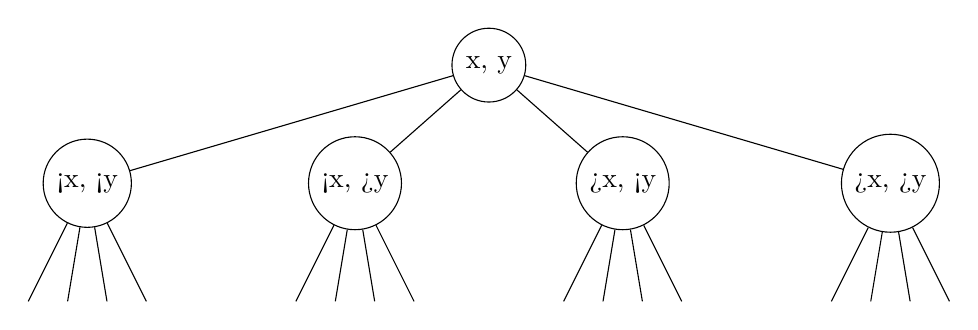
\begin{tikzpicture}
	[level 1/.style={sibling distance=34mm},
	level 2/.style={sibling distance = 5mm}]
	\tikzstyle{every node}=[circle,draw]
	\node {x, y}		
		child {
			node {<x, <y}
			child
			child
			child
			child
		}
		child {
			node {<x, >y}
			child
			child
			child
			child		
		}
		child {
			node {>x, <y}
			child
			child
			child
			child		
		}
		child {
			node {>x, >y}
			child
			child
			child
			child		
		}
	;
\end{tikzpicture}
	\caption{An illustration of the internal structure of the \texttt{Quadtree} data structure}
\end{figure}
\\
\subsubsection{FormatConverter class} % Converts from the data type pulled out of the data structure to the data type needed by the View package
The \texttt{FormatConverter} has static methods only, and only one public method. This methods takes an \texttt{ArrayList<Edge>} and converts it to the type \texttt{int[][][]} \\(\texttt{int[type][number of edges][edge coordinates]}).

The FormatConverter uses an instance of the Coordinates class to convert the given UTM32 coordinates to pixels as shown in the GUI.

\subsubsection{RoadDataCreator class} % Not directly part of the implementation, but the class used for converting the data from Krak to the krax XML format
The RoadDataCreator is not, strictly speaking, a part of the application (it is not used at runtime). It is a utility class, reading in the data supplied by Krak, writing it to an XML file of the KRAX format (once again using the external \href{www.xom.nu}{\texttt{xom}} library).

\subsubsection{The Graph}
Upon launching the application, the \texttt{Graph} class creates the two path finding graphs to be used by our path finding algorithm to find the fastest or the shortest path, respectively, between two given nodes.
	
The static \texttt{Graph} object itself contains \texttt{ArrayList} representations of each of these graphs. These will be referred to as graphs from now on. These graphs contain \texttt{Vertex} objects which have a position, some neighbouring vertices, and some adjacent edges (of the type \texttt{GEdge}). A \texttt{HashMap} for each of these two graphs is used to quickly access a vertex, given its id. Two \texttt{HashMaps} are used since each graph has its representation of each edge (the edges have different weights across the graphs). When searching for a path, the correct \texttt{ArrayList} and \texttt{HashMap} are returned, depending on whether the user requests the fastest path of the shortest path.

Furthermore, a third \texttt{HashMap} is used to keep track of each \texttt{Vertex's} adjacent \texttt{GEdges}.

\subsection{View package} % Consists of all the classes handling the graphical user interface
%The \texttt{View} package contains all the classes managing the graphical user interface.

\subsubsection{View class} % Front end class in the MVC pattern. Contains the rest of the (non-static) GUI classes. Implements the MapListener interface. The overall class structure of the View package
The \texttt{View} class is the front-end class of the \texttt{View} package in the MVC design pattern. It contains an instance of the \texttt{MainFrame} class, which is the basic \texttt{java.swing} GUI (the window to be displayed), which then again contains an instance of our custom panel, \texttt{MapPanel}.

The \texttt{View} itself implements the interface \texttt{ViewListener}, of which an instance is stored in both the \texttt{MainFrame} and the \texttt{MapPanel} classes. This allows for these classes to invoke a method in the \texttt{View}, telling it that changes has been made, which then invokes a similar method in the \texttt{Controller}, which then updates the GUI according the the changes.

\subsubsection{MapPanel class} % Draws lines according to input data
The \texttt{MapPanel} class extends the \texttt{java.swing.JPanel} class and functions as a panel with extended functionality and with an overridden \texttt{paint} method.

The \texttt{MapPanel} stores an \texttt{int[][][]} (as generated by the \texttt{FormatConverter}), from which it draws lines of the canvas, each corresponding to an edge stored in the \texttt{Model}. It also stores an instance of the \texttt{MapLocation} and \texttt{Trip} class (which both can be null), which are then drawn similarly to the roads, given that they are not null. The \texttt{MapLocation} is displayed as a filled circle, whereas the trip is displayed by drawing each of the road segments of which it consists.

The \texttt{MapPanel} also has two listeners from the \texttt{java.awt} library; a \\\texttt{MouseWheelListener}, which invokes a static method of the \texttt{ZoomHandler} class when the user scrolls on the panel, sending data about the mouse coordinates and the scrolled amount, and a \texttt{MouseMotionListener}, which invokes a static method of the \texttt{DragHandler} class when the user drags the mouse on the panel, letting the \texttt{DragHandler} know how far the mouse has been dragged (and along which axes).

\subsubsection{ZoomHandler class} % Handles all the zooming
The \texttt{ZoomHandler} handles all zooming. When a call is received (from the \texttt{MapPanel}), signaling that the user wishes to zoom out, there are two possible outcomes: If the current viewbox is not too close to the maximum width and height values; it zooms out, maintaining the current center of the viewbox. Otherwise, if the viewbox is near its extrema, zooming is done with the viewbox bound to the borders imposed by the maximum values.

Subsequently to zooming in, a call is made to the \texttt{DragHandler} class, moving the viewbox towards the current location of the cursor.

Zooming is simply a matter of changing the global values indicating what is being displayed (in the \texttt{MinAndMaxValues} class) / changing the size of the viewbox and then invoking a repaint of the \texttt{MapPanel}.

\subsubsection{DragHandler class} % Handles all the dragging
The \texttt{DragHandler} class, like the \texttt{ZoomHandler} class, changes the viewbox according to input data (drag amount and direction) and according the the maximum values that definine the extrema of the viewbox.

\subsubsection{SearchPanel class}
Like the \texttt{MapPanel} class, the \texttt{SearchPanel} class extends \texttt{javax.swing.JPanel}.

The \texttt{SearchPanel} contains components used for searching for addresses; two \texttt{JTextFields} allowing the user to input up to two addresses, two \texttt{JLists} for displaying proposed addresses to the user, two \texttt{JButtons}, one for executing a search for either a location corresponding to an address, or a search for a trip from one given address to another, two \texttt{JRadioButtons} in a \texttt{ButtonGroup} for toggling between searching for either the fastest or the shortest trip.

The \texttt{SearchPanel} else has several \texttt{JLabels}. Each component used for user interaction is labeled with explaining text. Below these components, there are label displaying the following info about the trip:
\begin{itemize}
 \item The distance of the trip in meters.
 \item The computed time of the trip in minutes.
\end{itemize}
given a such search has been executed recently (and a search for a location has not been made since).

All component listeners on the SearchPanel (be it ActionListeners, DocumentListeners etc.) either only affect things within the \texttt{SearchPanel} class or signals to the \texttt{SearchListener} (in this case the \texttt{View} class) to take action according to the input given by the user.

\subsection{AddressParser class}
The \texttt{ParseAddress} method is the basis of the \texttt{AddressParser} class. It uses regular expressions and pattern matching to parse an input address. The basic idea is that an input address can consist of up to three different "kinds" of parts:
\begin{itemize}
	\item Zero, one, or two city name / street name parts consisting of the characters allowed in them (i will reference to this as "\textit{name}").
	\item Zero or one zip code part consisting of digits (i will reference to this as "\textit{zip}").
	\item Zero or more parts containing the characters not allowed elsewhere, which allows the other parts to be determined from each other (i will reference to this as "\textit{other}").
\end{itemize}
The input \texttt{String} is matched with up to three different patterns (i will use the $\sharp$ as a separator. The words \underline{underlined} must be present, the rest are optional):
\begin{itemize}
	\item Pattern with the zip code last: \\
		\textit{other$\sharp$\underline{name}$\sharp$other$\sharp$name$\sharp$other$\sharp$zip$\sharp$other}
	\item Pattern with the zip code first \\
	\textit{other$\sharp$\underline{zip}$\sharp$other$\sharp$name$\sharp$other$\sharp$name$\sharp$other}
	\item Pattern with the zip code in the middle \\
	\textit{other$\sharp$\underline{name$\sharp$other$\sharp$zip}$\sharp$other$\sharp$name$\sharp$other}
\end{itemize}
If the first pattern matches, the city name, street name and zip code (or at least the parts found) are parsed to the format \textit{city name$\sharp$zip code$\sharp$street name}. If it doesn't match, the parser tries matching the input with the next pattern, parsing to the same format, and so on. If none of the patterns match, \texttt{null} is returned.

The \texttt{ParseAddressLive} method makes use of the \texttt{ParseAddress} method, but it cleans up the result for it to be optimal for doing a prefix search in the \texttt{TernaryTrie}. It removes any "empty" parts of the address which are in either the beginning or the end of the parse address. An example is the parsed address \textit{$\sharp$1234$\sharp$}, which will be cleaned to being simply \textit{1234}.

\subsection{Connecting the graphical user interface and the TernaryTrie}
The connection between the graphical user interface and the \texttt{TernaryTrie} makes use of the \texttt{Observer} design pattern. The \texttt{View} class implements the \texttt{SearchListener} interface, which contain methods to be invoked when the user interacts with the graphical user interface in a way, creating a need for classes other than the \texttt{SearchPanel} being active. The instance of the \texttt{View} class is stored in both the \texttt{SearchPanel} and the \texttt{MainFrame} classes.

Whenever the user types something in one of the text fields for inputting addresses (in the \texttt{SearchPanel} class), the following happens (as also illustrated in figure \ref{fig:autocompletion} on page \pageref{fig:autocompletion}):
\begin{itemize}
	\item A method \texttt{findOptions>>Number<<List()} (where \texttt{>>Number<<} is either \texttt{"First"} or \texttt{"Second"} depending on the text field being edited) in the \texttt{SearchListener} / \texttt{View} class is invoked.
	\item The input is parsed by the \texttt{AddressParser} class.
	\item The parsed string is passed to the instance of the \texttt{TernaryTrie} class stored in which a prefix search is done, finding all addresses having the parsed string as a prefix.
	\item The up to five first matches from the \texttt{TernaryTrie} are "cleaned" and stored in a \texttt{String[]} (this is done in the \texttt{cleanString} method which makes sure all letters start with a capitalized letter and that all words are comma and space separated (\texttt{", "})).
	\item The \texttt{String[]} is passed first to the \texttt{MainFrame} class, then to the \texttt{SearchPanel} class, which updates the content of the correct \texttt{JList} to display the \texttt{String[]}.
\end{itemize}
There is a special case, where the text field is empty (the user just deleted the only character(s)). In that case, the corresponding list below the text field is emptied, and nothing else happens.

\begin{figure}[!h]
\centering
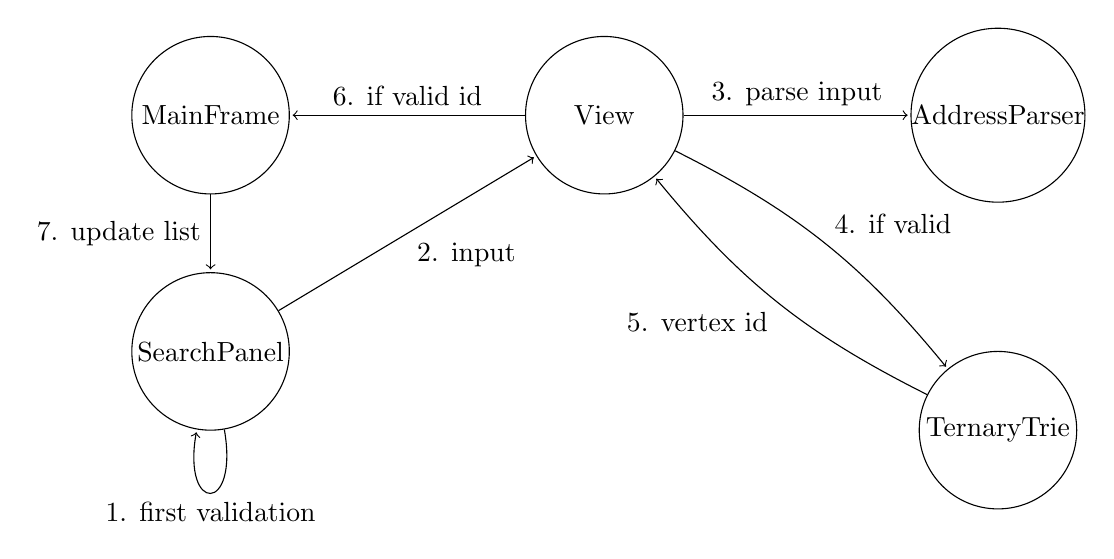
\begin{tikzpicture}
	\node [place, minimum size=2cm]	(SearchPanel)	at (0, 0) {SearchPanel}
		edge [in=-100, out=-80, loop] node[auto] {1. first validation} (SearchPanel);
	\node [place, minimum size=2cm]	(MainFrame)		at (0, 3) {MainFrame}
		edge [post] node [auto, swap] {7. update list} (SearchPanel);
	\node [place, minimum size=2cm]	(View)			at (5, 3) {View}
		edge [pre]	node [auto]	{2. input} (SearchPanel)
		edge [post] node [auto, swap] {6. if valid id} (MainFrame);
	\node [place, minimum size=2cm]	(AddressParser)	at (10, 3) {AddressParser}
		edge [pre] node [auto, swap] {3. parse input} (View);
	\node [place, minimum size=2cm]	(TernaryTrie)	at (10, -1) {TernaryTrie}
		edge [post, bend left=12] node [auto] {5. vertex id} (View)
		edge [pre, bend right=12] node [auto, swap] {4. if valid} (View);
\end{tikzpicture}
\caption{An illustration of the automatic input completion. It is simplified in the way that in some cases, two method calls a actually made by the \texttt{View} to the \texttt{TernaryTrie}.}
\label{fig:autocompletion}
\end{figure}

This process completely relies on the speed of the \texttt{TernaryTrie}, as the user would otherwise have to wait for all this to happen each time a character is type or removed.

\subsection{Connecting the graphical user interface and the \texttt{TernaryTrie} with the Model for searching for trips and locations}
Whenever the user presses the \texttt{"Find"} button (for executing a search), two things happen; First the address(es) are validated. If all needed addresses are valid, the search is executed in the \texttt{Model} package.

We will describe the process of searching for a location. The process of searching for a trip is the same, only it includes validating the contents of both input text fields and invoking a different method in the \texttt{Model} package.

The validity checking is a follows (as also illustrated on figure \ref{fig:ControlFlow} on page \pageref{fig:ControlFlow}):
\begin{itemize}
	\item The first address validation is done withing the \texttt{SearchPanel} class, checking that both of the input text fields are not empty, and if only the first is empty, the content of the second text field is moved to the first text field.
	\item The contents of the text field is sent to the \texttt{View}, where the vertex id corresponding to the given address is found.
	\begin{itemize}
		\item If the input itself, once parsed, is stored in the \texttt{TernaryTrie} with a corresponding vertex id, this is used.
		\item Else, a prefix search is done in the \texttt{TernaryTrie}, where the value of the first match is used as the vertex id.
	\end{itemize}
	\item If a vertex id is still not obtained / the input itself was not a match nor a prefix of any matches in the \texttt{TernaryTrie}, a warning message is displayed to the user informing that the input is invalid, and nothing more happens.
	\item If a vertex id is obtained, a method of the \texttt{ViewListener} (int the \texttt{Controller} class) is invoked, which again invokes a method in the \texttt{Model} class, obtaining an instance of the \texttt{MapLocation} class (storing the needed info about the location), which again is passed to the \texttt{View} class and from there to the \texttt{MapPanel} class, so it can be displayed to the user.
\end{itemize}

\begin{figure}[!h]
\centering
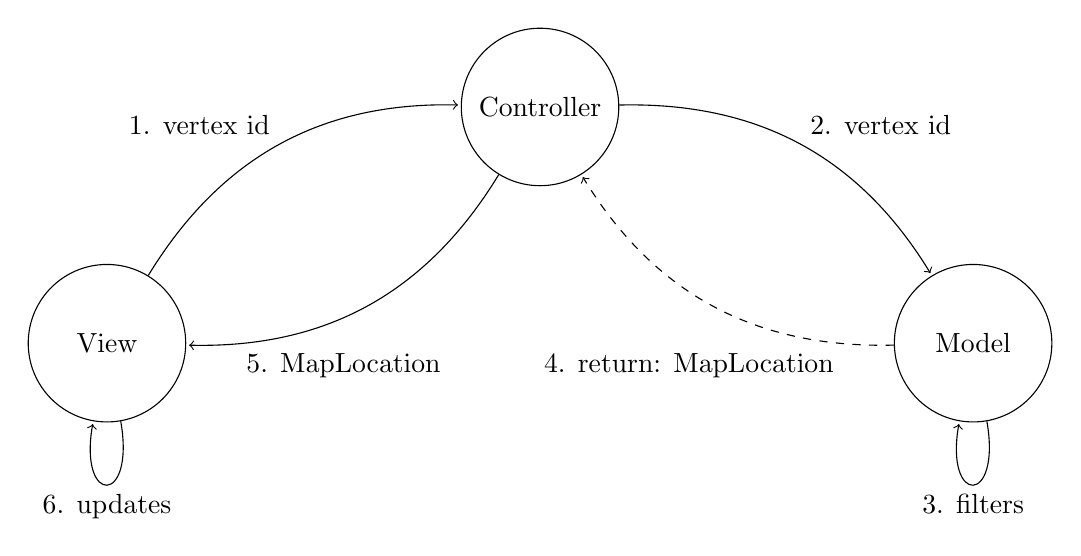
\begin{tikzpicture}
	\node [place, minimum size=2cm]	(View)			at (0,0)		{View}
		edge [in=-100, out=-80, loop] 	node [auto]	{6. updates} (View);
	\node [place, minimum size=2cm]	(Controller)		at (5.5,3)		{Controller}
		edge [pre, bend right=30]	node [auto, swap]	{1. vertex id}		(View)
		edge [post, bend left=30, very near end]	node [auto]	{5. MapLocation}		(View);
	\node [place, minimum size=2cm]	(Model)			at (11,0)		{Model}
		edge [pre, bend right=30]	node [auto, swap]	{2. vertex id}		(Controller)
		edge [post, bend left=30, dashed, very near start]	node [auto]	{4. return: MapLocation}		(Controller)
		edge [in=-100, out=-80, loop] 	node [auto]	{3. filters} (Model);
\end{tikzpicture}
\caption{An illustration of the flow of the application when a search for a location is executed. If the arrows of the text was changed, this would actually be a general illustration if the communication happening in all the processes within the application in which both the \texttt{Model} and the \texttt{View} packages are active.}
\label{fig:ControlFlow}
\end{figure}

\subsection{Use of external libraries}
The application makes use of the external package MigLayout (\texttt{net.miginfocom.swing.MigLayout}, \url{http://www.miglayout.com/}) for laying out the \texttt{javax.swing} components of the \texttt{SearchPanel} class. The library allows arranging the components relative to each other using a lot less code than would be necessary using the \texttt{layout managers} of the \texttt{java.awt} library.

\subsection{Use of "external" code}
A few of the classes of the application contains code which is not entirely written by ourselves. The classes \texttt{QuadTree}, \texttt{Interval}, and \texttt{Interval2D} are classes from \url{http://algs4.cs.princeton.edu/}, which is then modified to fit the needs of our application. The exact URLs / links to each of the classes are to be found as a comment within each of the classes, just below the imports.

The original classes generic of a type extending \texttt{Comparable}. Our modification extend to changing the generic type to be of the simple type \texttt{double}, allowing us to do comparisons using the \texttt{>}, \texttt{<}, and \texttt{==} operators and avoid auto-boxing and -unboxing.

Actually, the three classes were not compliant as they were first downloaded (or more exactly, the \texttt{Interval2D} class were not compliant with the others). But few modifications removed the issues. The logic of the code is still more or less exactly the same as it originally were.

!!! Missing information about from where the Dijkstra is found...

\subsection{Easter eggs}
\label{sec:Imp, Easter eggs}
The application includes two hidden features, so called easter eggs.

The first is concerning the input typed in by the user. The application allows the input being written as ASCII characters in binary, whereas the application will translate the input numbers to the corresponding address (similar to a regular search), once a search is executed.

The binary conversion, however, has its limitation. Since only ASCII characters are allowed, characters such as the "Nordic" letters are not allowed, or more precisely they are not possible to write. Also, the automatic text completion does not update the list of possible addresses while a binary input is typed by the user. This is, because the binary addresses are not stored withing the \texttt{TernaryTrie} class, but it is translated once the \texttt{Find}-button is pushed.

The second easter egg is that if the user types in the string "\textit{Rainbow Road}", trips will from there on be drawn using six different colors. For each road segment on the trip, a new color is used. Typing "\textit{Ordinary Road}" will reset the application to display trips in the default manner once again.

\subsection{Outline}
\begin{itemize}
	\item Include the sections from last report \\
		\textsl{Mikkel}
	\item Trie \\
		\textsl{Sigurt}
	\item Graphs \\
		\textsl{Niels}
	\item Connection between GUI and Trie and Graph \\
		\textsl{Mikkel}
	\item Use of external libraries \\
		\textsl{Mikkel}
	\item Use of "external" code \\
		\textsl{Mikkel}
	\item Easter-eggs \\
		\textsl{Mikkel}
\end{itemize}

\pagebreak
\section{Testing}
\label{sec:Testing}

\subsection{Outline}
\begin{itemize}
	\item Model package
	\begin{itemize}
		\item Coordinates \\
			\textsl{Blackbox testing of the \texttt{convertXToPixels} and \texttt{ConvertYToPixels} methods}
		\item Dijstra \\
			\textsl{Create one or two small sample graphs and run different path-findings with known results for testing}
		\item GVertex \\
			\textsl{Blackbox testing of the \texttt{distance} method}
		\item Vertex \\
			\textsl{Same as the GVertex \\Blackbox testing of the \texttt{distance} method}
		\item KrakToXMLConverter
			\textsl{Make a sample input with a know output and compare}
		\item QuadTree
			\textsl{Make a sample input with a know output and compare}
		\item TripEdge
			\textsl{Blackbox testing of the \texttt{computeTime} method}
	\end{itemize}
	\item View package
	\begin{itemize}
		\item AddressParser \\
			\textsl{Whitebox test of the different cases: zip first, zip middle, zip last, no match}
			\textsl{Blackbox test of a lot of different inputs}
		\item TernaryTrie \\
			\textsl{Make a sample input and do both prefix searches and value searches with known outcomes and compare}
		\item The graphical user interface
			\textsl{Testing the map, zooming, dragging etc. by trying it. Describe the testing and explain whether or not it is reasonably thorough}
	\end{itemize}
\end{itemize}


\pagebreak
\section{Discussion}
\label{sec:Discussion}

\subsection{Quadtree or k-D tree}
We have decided on a quadtree for our data structure. We believe that we could have got a similar result using k-D trees. The k-D trees have the advantage that they are easy to balance. Quadtrees have the advantage that they have an overall smaller height, due to the nature of the k-D trees being binary trees.

\subsection{Our use of four quadtrees}
Our current data structure consists of four quadtrees, one per type of edge stored. This means the application has to search through several quadtrees, if several types are to be drawn. It would be preferable having everything in the same tree, allowing the overall tree height (the sum of all our tree heights) to be smaller. But since we only have four quadtrees, we believe that the performance difference would be un-noticeable.

\subsection{Optimizing the Quadtree}
We thought about optimizing our QuadTrees such that when a sub tree is sufficiently small (say, contained a hundred elements) we would seize to further divide that sub tree and simply let store all these elements in an \texttt{Array} or some similar data type that would do the job. The reason for this is that recursion is not all that fast in \texttt{Java} and we might be able to achieve a faster data structure this way.

\subsection{Alternatives to the path finding algorithm}
Dijkstra's algorithm is not the fastest path finding algorithm and this does show when the paths get sufficiently long. Although it only takes about two seconds to find paths from one end of the map to another, this could very likely be improved by using another path finding algorithm such as the A* algorithm, which relies on heuristics to guess which direction to go in order to find a shortest path. We had some trouble implementing it, though, and working out a good heuristic for guessing the fastest path is not trivial as it cannot simply use the Manhattan distance (as would be the case when searching for the shortest path).

The graph still has a few flaws. For example, some paths between two arbitrary points A and B will look just fine when going from A to B, but when going from B to A, the algorithm will a completely useless path. We have not been able to figure out what the cause of this is.

\subsection{Memory usage}
The application stores a lot of information, which is read from several large text files at start-up. The information stored is for example information about each road segment in the quadtree data structure, each searchable address in different formats allowing the user to search efficiently with corresponding vertex ids, and a graph structure representing all the locations from the data from Krak and connections between them. The result is that the application already before any user interaction has been performed uses close to ??? of memory.

The memory uses is increased even further once the search for a trip is executed. A search, where the two given addresses are valid, results in the need of using extra space for the trip computation, bringing the memory usage up to about ???.

Another downside to all the information needed to be stored is the start-up time. It takes about ??? seconds on an average computer to launch the application. The major time consumers during the launch are the following: \\ \\
\begin{tabular}{ p{5cm} | p{3cm} }
	\textbf{Thing to be created} & \textbf{Launch time} \\
	\hline
	\texttt{QuadtreeDS} & ??? \\
	\texttt{Graph} & ??? \\
	\texttt{TernaryTrie} & ??? \\
	\texttt{Graphical user interface} & ???
\end{tabular}
\\ \\ \\
If the application were to be distributed, ??? seconds is a quite long start-up time for an application. And since the application shows no information to the user about the progress of the application, the user might think that the application has not started to launch at all. In the worst case, the user could then try to run the application multiple time, which would result in an even larger usage of memory, and with an average personal computer, the memory usage would most likely try to exceed the physical limits.

Even that standard memory usage of the application will use up such a vast amount of memory on the computer on the user that running other applications simultaneously with running this application would most likely be a slow experience, given the application is running on an average personal computer.

We do, however, believe that the upsides to the memory usage by far exceeds the downsides. To be more exact, it would not be possible for the application to run as it does, were the information not stored in the memory of the computer, since the application is based on data structures optimized for searching in different ways.

An alternative to having such a vast memory usage on the computer of the user could be a client-server situation, where all the information is stored in the memory of the server, allowing for optimized searches, whereas the client side needs only the very small part of the information which is currently to be displayed in the graphical user interface. This would moreover open up for the possibility of have more than one client accessing the same server simultaneously. But it was a design decision of ours having everything within the application and thereby also making the application accessible by only one user at the time, e.g. the user on the computer itself. Having it any other would, as mention in ??? demand changes to the overall structure of the application.

\subsection{Easter eggs}
The easter eggs of the application as described in section \ref{sec:Imp, Easter eggs} og page \pageref{sec:Imp, Easter eggs} does not really add anything to the application itself from the user's point of view. However, we decided to include them anyway because the add a lot to the application from our point of view as the makers of the application.

More or less as soon as we had implemented the finding of trips, the implementation of the \textit{Rainbow Road} easter egg was implemented as well (actually this was through most of the writing of the application the default way of displaying roads with no other options available). And it is something we have actually had quite a lot of fun with. We find it unnecessary or at least sad to remove a, though small, part of the application which has been essential to the process of making the application. Instead we decided to hide it as an easter egg.

The \textit{Binary Input} easter egg has not, like the \textit{Rainbow Road}, been a part of application for a long time. The main reasons for having this hidden feature is that it is the only feature supported by our application, which is not supported by the major providers of map services.

\subsection{Outline}
\begin{itemize}
	\item Platform - Must be expanded to include slow search etc. \\
		\textsl{Jacob}

                *****I do not understand what is meant with this one?****

                

	\item Quadtree or k-D tree \\
		\textsl{Done}
	\item Optimizing the quadtree \\
		\textsl{Niels}
	\item Disappearing roads \\
		\textsl{Jacob}

                We have been experiencing some disappearing roads while viewing the map at a zoom level where we see all road types. This is due to the way our data structure is made, and we did not discover this problem in time to change the data structure and fix the problem entirely. Fortunately it is only very long edges that disappear at certain zoom levels. The only edges that we have really experienced this problem with, are the fairy roads. When a road disappears it happens because none of the nodes of the edge is in the "viewbox" of the program. When we zoom in we need to know which roads to draw in the frame. This is done my checking if the coordinates of an edge's nodes is within the "viewbox" or its buffer zone. If neither of the nodes are withing the zone, the edge is not drawn. So naturally when a very long edge should be drawn in the "viewbox", but does not have any of its nodes in the zone it is not drawn. 

	\item Running path-finding in a separate thread \\
		\textsl{Jacob}
		
		For quite a long period we had some great troubles making the path-finding searches using Dijksta's algorithm. A single search could easily take more than 30 seconds to finish. We had very big troubles figuring out what caused this slow search. We tried implementing the A* algorithm instead, but without any luck. Due to this slow search we started looking at the opportunity to make the path-finding run in a separate thread, giving the user the possibility to still navigate and explore the map. 

		This was, however, after a meeting with Rasmus Pagh, not a problem anymore, since we found out that the priority queue that our Dijkstra implementation used was very slow and actually running in linear time when removing things. By deleting the part of the implementation where the non-fastest roads are removed from the priority queue, our path-finding search was now done in less than 0.5 seconds, and we did no longer see any reason to run the path-finding in a separate thread.

	\item Landscape drawing \\
		\textsl{Jacob}

		To make the map look a lot better and give a better idea of what part of the map the user is looking at, we would have liked to add some landscape and coastlines to the map. This did however not have a very high priority. 

		To retrieve some data that we could possibly use to draw some landscape and coastlines, we wrote an email to krak.dk/eniro.dk and asked whether we could have the data files that they use for their own map. After a couple of emails back and forth, we were given the address to an ftp server from where we could download all the data that Krak themselves use for their map service. Unfortunately the data types were not of the same type that the types we use, and we did not have the time to make the new data type work with our own. Since it is not vital for our program, and the program still serves its purpose we did not add landscape.

	\item Alternatives to our path-finding algorithm \\
		\textsl{Niels}
	\item Incorrect paths found \\
		\textsl{Niels}
	\item Finding a city only \\
		\textsl{Sigurt}
	\item Encoding \\
		\textsl{Sigurt}
	\item Reading the XML-file as a text file \\
		\textsl{Mikkel}
	\item Memory usage \\
		\textsl{Mikkel}
	\item Easter eggs \\
		\textsl{Mikkel}
\end{itemize}


\pagebreak
\section{Reflection}
\textsl{Sigurt}
\begin{itemize}
	\item Communicating through Facebook
	\item Technical issues (Skype) - Meeting in person instead
	\item Balance between working as a group and working separately
	\item Delegation of responsibilities - Issues with different modules not interacting perfectly
	\item The meetings
	\item Use of the constitution
	\item Use of a project diary
	\item Overall
\end{itemize}


\pagebreak
\section{Conclusion}
\label{sec:Conclusion}


\pagebreak
\appendix
\section{Group constitution}
\underline{Organization} (e.g. joint, distributed, other?) \\
We aim towards a mixture of the three. Working in plenum when neccessary, but retaining the possibility to distribute work when we see it fit. \\ \\
\underline{Work} (e.g. when, how much, sprinting/jogging?) \\
Meetings scheduled for monday.
Extra meetings will be planned ad-hoc \\ \\
\underline{Being together} (e.g. disagreement resolution, \ldots) \\
We will solve problems by dispute. Only when agreement is not an option will decissions be made by vote.

If agreement cannot be reached, even by vote, we will seek counsel from our teacher or TA. \\ \\
\underline{Managin differences in ambitions, \ldots} \\
We will try to maintain the highest possible level of ambition. \\

\pagebreak
\section{Project diary}

\subsection{Monday, 19/3-2012}

\hiddensubsubsection{Agenda}
\begin{enumerate}
	\item Platform decision - SVG or Swing
	\item Versioning
	\item IDE?
	\item Set up verisoning
	\item Report-writing
	\item How to get started
\end{enumerate}
\underline{1. Platform decision} \\
Will have decided using Java Swing. \\ \\
\underline{2. Versioning} \\
We will use git, since some group members are familiar with it. \\ \\
\underline{3. IDE?} \\
Eclipse is our decision. \\ \\
\underline{4. Set up versioning} \\
This is mostly done (it is done on most of our computers. The repository is working). \\ \\
\underline{5. Report writing} \\
We will write the repot in LaTeX.

\hiddensubsubsection{Reflection}
\underline{Discussion of the main class structure (packages):}
\begin{itemize}
	\item Controller \\
		\textsl{Controller (main class)}
	\item View \\
		\textsl{MapPanel} \\
		\textsl{MainFrame} \\
		\textsl{View} \\
		\textsl{ViewListener}
	\item Model \\
		\textsl{Edge} \\
		\textsl{DataFilter} \\
		\textsl{KrakToXMLConverter} \\
		\textsl{Model} \\
		\textsl{XMLReader}
\end{itemize}
\underline{Other} \\
Our krak-data to XML converter from a previous assignment has been remade to include a "type" element

The XMLReader works on small XML files

At all points there is a general agreement.
We have decided to start by making a simple visualization, then improving the functionality step by step, making sure the basic implementations work as they should.

\hiddensubsubsection{Work sheets}
\begin{itemize}
	\item The XMLReader is currently exceeding heap space \hfill \\
		\textsl{Niels will try to fix this}
	\item Read about k-d trees \hfill \\
		\textsl{Think about the possibility of using it as our main data structure}
\end{itemize}

\hiddensubsubsection{Next meeting}
Wednesday, 19/3-2012, 18:30

\pagebreak
\subsection{Wednesday, 21/3-2012}

\hiddensubsubsection{Agenda}
\begin{enumerate}
	\item Analyze the current problems
	\item Who does what
	\item Testing
\end{enumerate}
\underline{1. Analyze the current problems} \\
Our first step will be reading in the entire map-data and drawing it according to the class diagram \\ \\
\underline{2. Who does what} \\
According to the "work sheets" \\ \\
\underline{3. Testing} \\
When a class is created/implemented for which it is obvious that a JUnit test is suitable, this will as far as possible be created alongside with the class/implementation

\hiddensubsubsection{Reflection}
We are currently in the need of a good overview allowing us to hand out assignments properly. The result is that we have a hard time all working at the same time.

We will try making a proper interface / maybe an UML-diagram showing the result of our current analysis and discussions.

\hiddensubsubsection{Work sheets}
\begin{itemize}
	\item XMLReader modified \hfill \\
		\textsl{Niels will do this}
	\item Build the base structure of the Model class \hfill \\
		\textsl{Mikkel will do this (difficult to be more than one person doing it)}
	\item Establish the communication between the Model/View/Controller \hfill \\
		\textsl{Mikkel will do this (same as last)}
	\item Create class in the Controller package with a static method to convert an ArrayList<Edge> into a proper int[][][] for the MapPanel class. \hfill \\
		\textsl{Sigurt and Jacob got this one!}
\end{itemize}
\underline{Implementations waiting to be done:} \\
\begin{tabular}{| p{3cm} | p{4cm} | p{5cm} |}
	\hline
	DataFilter & FilterData(edges, minX, maxX, minY, maxY) & Filters the given data according to the given parameters \\
	\hline
	FormatConverter & convertData(Array-List<Data> edges) & Converts the ArrayList<Edge> into a proper int[ ][ ][ ] for the MapPanel \\
	\hline
	View and MapPanel & viewboxUpdated(???) & Tells the view that a new ?viewbox? is set.
We need to figure out the right parameters \\
	\hline
	XMLReader & readXML() & Needs to be implemented to work with the Model class \\
	\hline
	MapPanel & Something allowing to update the viewbox and call the viewboxUpdated-method & Next step. First, we need to visualize the entire map \\
	\hline
	
\end{tabular}

\hiddensubsubsection{Next meeting}
Monday, 26/3-2012

\pagebreak
\subsection{Monday, 26/3-2012}

\hiddensubsubsection{Agenda}
\begin{enumerate}
	\item Class structure
	\item Structure of FormatConverter
	\item Who does what
	\item Implementation
\end{enumerate}

\hiddensubsubsection{Reflection}
We now have a (hopefully) working implementation of our data structure, but we are still without filtering of edges.

Our application can now draw the entire map on a custom JPanel, but still no filtering is done, and zooming causes errors.

We have spend a lot of time on technical issues with versioning and Eclipse.

\hiddensubsubsection{Work sheets}
\begin{itemize}
	\item Go from using ArrayList<Edge> to KDTree. This requires changes in several classes \\
		\textsl{Niels and Jacob}
	\item Filtering data according to coordinates and type \\
		\textsl{Niels and Jacob}
	\item Zooming \\
		\textsl{Mikkel and Sigurt}
	\item Panning
	\item Report
\end{itemize}
We don?t expect anything to be done till next time, but we are going to take a look at the differing subjects above

\hiddensubsubsection{Next meeting}
Wednesday 28/3-2012, at ITU, 17:00

\pagebreak
\subsection{Wednesday, 28/3-2012}

\hiddensubsubsection{Agenda}
\begin{enumerate}
	\item Data structure
	\item MapPanel
\end{enumerate}
Today is following the class structures we have made previously. We are going to work with the implementations. \\ \\
\underline{1. Data structure} \\
We are currently working on a custom-implementation of a kd-tree, but it is causing many difficulties. Most of the work to follow will be concerning this \\ \\
\underline{2. MapPanel (The visualization of the data)} \\
We now have decent zoom- and panning-capabilities, and everything runs fairly well (considering it is running on a ?mock?-implementation of our data structure). One last modification concerning zoom coordinates is to be made.

\hiddensubsubsection{Reflection}
We are having many difficulties concerning the kd-tree, which might be because we have not completely understood how we can use it / how to make it the base of our storage of data.

We continue having a very relaxed tone at our group meetings, were were discuss issues (the only issues are really about the project) as they come.

We all feel that we are moving towards a result we are very satisfied with.

\hiddensubsubsection{Work sheets}
\begin{itemize}
	\item Implement the last needed zoom capability \\
		\textsl{Mikkel will do this}
	\item Make the kd-tree replace the mock-implementation of our data structure \\
		\textsl{Niels work on this}
	\item Start making descriptions of our project / parts of the report \\
		\textsl{Jacob might look into this if he finds the time}
\end{itemize}

\hiddensubsubsection{Next meeting}
Monday, 2/4-2012, 10:00


\pagebreak
\subsection{Monday, 2/4-2012}

\hiddensubsubsection{Agenda}
\begin{enumerate}
	\item Do we have questions for Rasmus?
	\item Discuss data structure
	\item How should window resizing work
	\item Are we missing any part of the implementation
	\item Testing
	\item Report
\end{enumerate}
\underline{1. Do we have questions for Rasmus?} \\
We had and asked a question about balancing QuadTrees. We got an acceptable answer and tested balanced vs unbalance QuadTrees and decided to go with unbalanced. \\ \\
\underline{2. Discuss data structure} \\
We decided on using a QuadTree, since the implementation was already working. \\ \\
\underline{3. How should window resizing work} \\
We tried keeping a constant width / height ratio, but it worked poorly on the Linux computers. Now the window is only resized according to the most significant of x or y. \\ \\
\underline{4. Are we missing any part of the implementation} \\
Currently, nothing is missing. The rest has been implemented today. \\ \\
\underline{5. Testing} \\
We have made test classes for the classes to which it seemed fair to test that way. \\ \\
\underline{6. Report} \\
We have made an outline for the report. We have split the report into three parts after discussion (other than introduction and conclusions). As earlier decided, the report is written in a LaTex document, which is part of our git repository. The outlines of each section is in the document. The layout is done as well. \\ \\

\hiddensubsubsection{Reflection}
We are all very satisfied with the product as it currently is.
We have (quite easily) come to agreement about the contents of the report.
We are aware that we will need time making the report homogeneous.
The works sheets are due to tomorrow (next meeting) as far as possible.

\hiddensubsubsection{Work sheets}
\begin{itemize}
	\item Cleanup \\
		\textsl{Mikkel}
	\item UML (after cleanup) \\
		\textsl{Sigurt}
	\item Javadoc \\
		\textsl{Niels}
	\item Design choices (report section) \\
		\textsl{Jacob}
	\item Implementation (report section) \\
		\textsl{Mikkel}
	\item Discussion / reflection (report section) \\
		\textsl{// Wait 'til later}
\end{itemize}

\hiddensubsubsection{Next meeting}
Tuesday 3/4-2012, 19:00


\pagebreak
\subsection{Tuesday, 3/4-2012}

\hiddensubsubsection{Agenda}
\begin{enumerate}
	\item The sections of the report already written
	\item What to do with the rest of the report
\end{enumerate}
\underline{1. The sections of the report already written} \\
They need to be corrected / spellchecked (One person will run through the entire report in the end), but they are written to a satisfying level and will not need major changes. \\ \\
\underline{2. What to do with the rest of the report} \\
The introduction and conclusion will be written by the same person, so they are alike. One person will write the Discussion section.

\hiddensubsubsection{Reflection}


\hiddensubsubsection{Work sheets}
\begin{itemize}
	\item Introduction and conclusion \\
		\textsl{Jacob}
	\item Discussion \\
		\textsl{Mikkel}
\end{itemize}

\hiddensubsubsection{Next meeting}
Sunday 8/4/12 1001 hours via Skype

\hiddensubsubsection{Note}
\begin{itemize}
	\item Unspecified exception in Model class
\end{itemize}


\pagebreak
\subsection{Sunday, 8/4-2012}

\hiddensubsubsection{Agenda}
\begin{enumerate}
	\item Look through newly written parts of the report
\end{enumerate}
\underline{1. Look through newly written parts of the report} \\
Only minor corrections have been made

\hiddensubsubsection{Reflection}
The current task are very small, and we are very close to being done.

\hiddensubsubsection{Work sheets}
\begin{itemize}
	\item Correct the entire report \\
		\textsl{Sigurt}
	\item Shorten the Implementation and Discussion sections \\
		\textsl{Sigurt}
	\item Specify the Exception in the Model class \\
		\textsl{Niels}
	\item Have a final look through the source code \\
		\textsl{Niels and Mikkel}
\end{itemize}

\hiddensubsubsection{Next meeting}
Tuesday 10/04-2012, 17:00 at ITU


\pagebreak
\subsection{Tuesday, 10/4-2012}

\hiddensubsubsection{Agenda}
\begin{enumerate}
	\item Look through the report
	\item Make a jar file
	\item Organize the source code
	\item Make pdf with the report
	\item Send the entire assignment
\end{enumerate}

\hiddensubsubsection{Reflection}
Everything is finished, though it took a bit longer time than first expected.

We has issues with creating executable .jar files, which would work on the computers running Mac OS X (no issues on Arch Linux and Windows). However, when avoiding using Java 7 (as it is not yet available for Mac) and by running the .jar file from command line allowing it to use at least 256mb memory, everything works on Mac as well.

Everything is now handed in.

\hiddensubsubsection{Work sheets}
Nothing until the next part of the assignment is given.

\hiddensubsubsection{Next meeting}
Monday 16/4-2012, after the lecture.


\pagebreak
\subsection{Monday, 16/4-2012}

\hiddensubsubsection{Agenda}
\begin{enumerate}
	\item Appointments with TA / Rasmus
	\item Plan the future
	\begin{enumerate}
		\item Design decisions
		\item Make well-defined work sheets
	\end{enumerate}
	\item Get started
\end{enumerate}

\hiddensubsubsection{Reflection}
A list of fairly well defined work sheets has been made.

Along with each assignment (work sheet), we have agreed to write part of the report concerning the assignment, containing:
\begin{itemize}
	\item Design decisions
	\item Implementation
	\item Discussion
\end{itemize}

\hiddensubsubsection{Work sheets}
\begin{itemize}
	\item The search GUI \\
		\textsl{Mikkel}
	\item Auto completion \\
		\textsl{Sigurt}
	\item Draw the fastest / shortest path \\
		\textsl{Mikkel}
	\item Dynamic road resizing \\
		\textsl{Mikkel}
	\item Compute the shortest / fastest path \\
		\textsl{Jacob and Niels}
\end{itemize}

\hiddensubsubsection{Next meeting}
Wednesday 18/4-2012, 17:00 at ITU


\pagebreak
\subsection{Wednsday, 18/4-2012}

\hiddensubsubsection{Agenda}
\begin{enumerate}
	\item Work day
	\item Recap
\end{enumerate}

\hiddensubsubsection{Reflection}
We have decided to end the meeting at 19:30.

The graph structure is finished buts needs to be integrated in the rest of the application

The graphical user interface is progressing.

The overall flow of the application is currently being expanded to include the new features.

Work on the  ?street name lookup system? seems to be progressing.

\hiddensubsubsection{Work sheets}
Same as last time

\hiddensubsubsection{Next meeting}
Monday 23/4-2012, 10:00 at ITU


\pagebreak
\subsection{Monday, 23/4-2012}

\hiddensubsubsection{Agenda}
\begin{enumerate}
	\item Match the modules
	\begin{enumerate}
		\item The graph
		\item the user interface
		\item the trie
	\end{enumerate}
	\item File containing the graph info
	\begin{enumerate}
		\item Format: \textsl{id,x,y otherId otherId otherId \ldots}
	\end{enumerate}
	\item File containing the trie info
	\begin{enumerate}
		\item Format: \textsl{Something$\sharp$Something else$\sharp$Something else;nodeId}
	\end{enumerate}
\end{enumerate}

\hiddensubsubsection{Reflection}
We have spend quite a lot of time discussing how to make the different ?modules? of the application that we have created fit together.
The result of the discussion was a solution, which we then started working on (seperate people working on seperate parts of the solution).

The solution is not currently finished, but we are quite certain, that it will work properly.

The issues were as following:
\begin{itemize}
	\item The interfaces of the class for finding shortest paths and the classes allowing the user to search for addresses were not compliant
\end{itemize}

The solution is as following:
\begin{itemize}
	\item All the valid addresses are store in a trie (several addresses / ways of typing an address are stored and referenced to the same ids).
	\item We will pre-compute a file containing the graph structure, allowing for it to be read when the application starts, whereas it will be stored in a field. The field is then used when finding shortest paths.
	\item The graph will support shortest-path queries of the following form: pathTo(int nodeID, int nodeID). The trie stores the addresses and their corresponding nodeID.
\end{itemize}

\hiddensubsubsection{Work sheets}
\begin{itemize}
	\item Finishing the trie \\
		\textsl{Sigurt will \textsl{try}}
	\item Add validation to / finish the application creating the file containing the trie data \\
		\textsl{Mikkel}
	\item Optimize the graph (making it usable) \\
		\textsl{Niels}
	\item Reach max level in the Diablo III beta \\
		\textsl{Jacob}
\end{itemize}

\hiddensubsubsection{Next meeting}
Wednesday 25/04-2012, 17:00 at ITU


\pagebreak
\subsection{Wednesday, 25/4-2012}

\hiddensubsubsection{Agenda}
\begin{enumerate}
	\item Make a proper graph file
	\item Make the graph respond with the rest
	\item Test (and fix) the Trie file
	\item Make the Trie talk with the Trie file
\end{enumerate}

\hiddensubsubsection{Reflection}
Deadline:\quad 20:00

The finding of shortest paths is functional, but the graph needs a seperate class.

The trie is functional, and so is the address parser we will use. We will need to make them interact.

There are currently issues with the trie file, as it stores each city many times. This must be fixed.

We are having issues with Eclipse using different character encodings on our different machines. We will need to coordinate changing to the same format the next time we meet.

\hiddensubsubsection{Work sheets}
\begin{itemize}
	\item Create a seperate class for the graph \\
		\textsl{Niels}
	\item Make interaction between the GUI, trie, and the model \\
		\textsl{Mikkel}
	\item Fix issues with the trie data file \\
		\textsl{Sigurt (look at line 162)}
	\item Get well \\
		\textsl{Jacob (done)}
\end{itemize}

\hiddensubsubsection{Next meeting}
Sunday 29/4-2012, 12:00 at ITU


\pagebreak
\subsection{Monday, 30/4-2012}

\hiddensubsubsection{Agenda}
\begin{enumerate}
	\item What to do with the meeting with Filip
	\item What to do with the meeting with Rasmus
	\item How far are we
	\item What are we missing
	\item Decide on extras
\end{enumerate}
\underline{1, What to do with the meeting with Filip} \\
We will meet with Filip on Wednesday, 2/5-2012 at 10 am. \\ \\
\underline{2. What to do with the meeting with Rasmus} \\
We will write a mail to Rasmus, hoping to be able to discuss extensions on Monday, 7/5-2012. Hopefully this will be possible after 11 am, so all group members can take part. \\ \\
\underline{3. How far are we} \\
The project currently passes the minimum requirements. \\ \\
\underline{4. What are we missing} \\

\underline{5. Decide on extras}
\begin{enumerate}
	\item Description of the route
	\item Coastline / landscape
	\item Displaying the road names
	\item Choose transportation type
\end{enumerate}

\begin{enumerate}
	\item Feries
	\item Improve the trie data
	\item Improve the speed of the path-finding
	\item Find quickest path, not only shortest
	\item Make the screen move to what is found
	\item Take care of commas in the street name of the Krak data
	\item Splash screen for the long loading time
\end{enumerate}

\hiddensubsubsection{Reflection}
The improvement on the path finding is currently not working. We have started using a new algorithm. We will need more time working on this.

The trie data is fine now (we think).

Making the screen move correctly is not as trivial is hoped and will take some more time.

\hiddensubsubsection{Work sheets}
\begin{itemize}
	\item Write to Filip and Rasmus \\
		\textsl{Mikkel}
	\item Feries \\
		\textsl{Mikkel (not first priority)}
	\item Trie data \\
		\textsl{Sigurt}
	\item Speed of path finding \\
		\textsl{Niels and Jacob}
	\item Edge weight by time (not length) \\
		\textsl{Niels and Jacob}
	\item Move the screen when searching \\
		\textsl{Mikkel}
	\item Clean up the shared folder \\
		\textsl{Sigurt}
	\item Splash screen
\end{itemize}

\hiddensubsubsection{Next meeting}
Niels and Mikkel will meet with Filip Wednesday 2/5-2012, 10.00 at ITU.
Next group meeting: \\
Thursday 10.00, 3/5-2012 at ITU


\pagebreak
\subsection{Thursday, 3/5-2012}

\hiddensubsubsection{Agenda}
\begin{enumerate}
	\item What \underline{needs} to be done
	\item Plan the meeting with Rasmus on Monday
	\item Outline the report (12:00)
\end{enumerate}
\underline{1. What needs to be done} \\
\begin{itemize}
	\item Fastest path (done)
	\item Trie data
	\item Zoom to the right location (semi-done. It works, but currently is does not check if the location is too close to the ?borders?)
	\item Testing (what can be tested)
\end{itemize}
\underline{2. Plan the meeting with Rasmus} \\
\begin{itemize}
	\item The length of the report \\
		\textsl{It is fine if it is short}
	\item The roads ?disappearing? when dragging (since we check only for edge end coordinates) \\
		\textsl{Discussion of how it could be done}
	\item Optimising the quadtree
	\item Running path-finding in a separate thread
	\item Global package
	\item Landscape drawing
	\item Displaying road names
	\item a*
	\item Different ways to transport
	\item Route description
\end{itemize}
\underline{3. Outline the report} \\
Done somewhere else. \\ \\

\hiddensubsubsection{Reflection}
Issues:
\begin{itemize}
	\item Somewhere old ?dropdown lists? are stored, which are interfering with the searches.
	\item We have issues concerning the application getting slower. We need to look at some garbage collection.
	\item The displayed time is incorrect - Should be stored as double.
\end{itemize}
We have decided to ?stop? implementing (finishing) on Monday 7/5-2012.
After that day, we will finish the report before continuing the work on the implementation.

\hiddensubsubsection{Work sheets}
\begin{itemize}
	\item Testing / what can we test \\
		\textsl{Jacob}
	\item Trie data and JLists \\
		\textsl{Sigurt}
	\item Including the fastest path search in the application \\
		\textsl{Mikkel}
	\item Issues \\
		\textsl{Niels}
	\item Consider if we miss anything in the Design decisions section of the report \\
		\textsl{Everyone}
\end{itemize}

\hiddensubsubsection{Next meeting}
Monday 7/5-2012, 11:00 at ITU


\pagebreak
\subsection{Monday, 7/5-2012}

\hiddensubsubsection{Agenda}
\begin{enumerate}
	\item Prepare for the meeting with Rasmus
	\item Finish / fix the critical problem
	\item How to write the report
	\item Testing
\end{enumerate}

\hiddensubsubsection{Reflection}
The meeting with Rasmus went well. We got the information we needed and we are close to the planned implementation stop.

We are still missing a lot of testing.

\hiddensubsubsection{Work sheets}
\begin{itemize}
	\item Clean up memory? \\
		\textsl{Niels}
	\item Faster PQ (remove method) \\
		\textsl{Done. Our path-finding is quite fast now (though it uses some memory)}
	\item Trie data \\
		\textsl{Sigurt}
	\item Issue: Sometimes the point from which a path is found can not be changed \\
		\textsl{Jacob}
	\item Insert project diaries into the report \\
		\textsl{Mikkel}
\end{itemize}
All the work sheets for this day will be completely finished for next meeting, where we will start writing the report.

\hiddensubsubsection{Next meeting}
Thursday 10/5-2012, 10:00 at ITU


\pagebreak
\subsection{Thursday, 10/5-2012}

\hiddensubsubsection{Agenda}
\begin{enumerate}
	\item Discuss the application as it currently is
	\item Outline / discuss the report (12:00)
\end{enumerate}

\hiddensubsubsection{Reflection}
We have reached the implementation stop. We are currently focusing on the report. Some things are still missing in the implementation, but for now they will be discussed in the report rather than being fixed. If we have time later (when the report is finished), we might look at the issues again.

The report has been outlined (in the LaTeX document), and each section has been assign to a group member. In order for us to have time to evaluate our report in several stages of the writing process, we will finish the draft of the report for the next meeting (in three days), where we will discuss it.

We will write to Filip, hoping that he has the time to look at the report draft and discuss it.

\hiddensubsubsection{Work sheets}
\begin{itemize}
	\item Write the sections / report
\end{itemize}

\hiddensubsubsection{Next meeting}
Sunday 13/5-2012, 10:00 at ITU

\pagebreak
\section{Work sheets made on Monday, 17/4-2012}


\pagebreak
\section{Testing}

\subsection{AddressParser class}
The testing of the \texttt{parseAddress} method of the \texttt{AddressParser} class includes a whitebox test and a blackbox test. The whitebox test consists of input data sets from the blackbox testing, making the two tests share a single expectancy table.

\subsubsection{Whitebox test of the parseAddress method}
\begin{tabular}{ p{7cm} | p{4cm}}
	\textbf{Input property} & \textbf{Input data set} \\
	\hline
	Zip code last match & ??? \\
	Zip code middle match & ??? \\
	Zip code first match & ??? \\
	No match & ???
\end{tabular}

\subsubsection{Blackbox test of the parseAddress method}


\subsubsection{Shared expectancy table}

\pagebreak
\subsection{Coordinates class}
For the testing of both of the following methods, the values of the \texttt{MinAndMaxValues} class, which are used are set to the following:
\begin{itemize}
	\item $minX = 20$
	\item $maxX = 120$
	\item $minY = 30$
	\item $maxY = 130$
	\item $width = 10$
	\item $height = 10$
\end{itemize}

\subsubsection{Blackbox test of the \texttt{convertXToPixels method}}
The \texttt{convertXToPixels} methods has been tested according to the following expectancy table: \\ \\
\begin{tabular}{ p{3.5cm} | p{2.5cm} | p{2.5cm} | p{2.5cm} }
	Input property & Input & Expected output & Actual output \\
	\hline
	Ordinary number & 50 & 3 & 3 \\
	Minimum value & 20 & 0 & 0 \\
	Maximum value & 120 & 10 & 10 \\
	Lower than minimum & 10 & -1 & -1 \\
	Higher than maximum & 130 & 11 & 11
\end{tabular}

\subsubsection{Blackbox test of the \texttt{convertXToPixels method}}
The \texttt{convertYToPixels} methods has been tested according to the following expectancy table: \\ \\
\begin{tabular}{ p{3.5cm} | p{2.5cm} | p{2.5cm} | p{2.5cm} }
	Input property & Input & Expected output & Actual output \\
	\hline
	Ordinary number & 60 & 7 & 7 \\
	Minimum value & 30 & 10 & 10 \\
	Maximum value & 130 & 0 & 0 \\
	Lower than minimum & 20 & 11 & 11 \\
	Higher than maximum & 140 & -1 & -1
\end{tabular}

\pagebreak
\subsection{Dijkstra class}

\pagebreak
\subsection{GVertex and Vertex classes}
Both the \texttt{GVertex} and \texttt{Vertex} classes share the \texttt{distance} method, only taking different parameters. Both methods have been blackbox tested according to the following expectancy table: \\ \\
\begin{tabular}{ p{3.5cm} | p{2.5cm} | p{2.5cm} | p{2.5cm} }
	Input property & Input & Expected output & Actual output \\
	\hline
	Positive numbers, increasing & $(8,4$), $(16,12)$ & $11.3137$ & ??? \\
	Positive numbers, decreasing & $(20,15)$, $(13,12)$ & $7.6158$ & ??? \\
	Positive numbers, one coordinate increasing, one decreasing & $(10, 5)$, $(5, 10)$ & $7.0711$ & ??? \\
	Negative numbers & $(-10, -3)$, $(-3, -1)$ & $7.2801$ & ??? \\
	Negative and positive numbers & $(7, 5)$, $(-7, -5)$ & $17.2047$ & ??? \\
	Positive and negative numbers mixed & $(1, -3)$, $(17, 2)$ & $16.7631$ & ??? \\
	All numbers zero & (0, 0), (0, 0) & 0.0000 & ??? \\
	One number zero & (0, 0), (-3, 7) & $7.6158$ & ??? \\
	Decimal numbers & $(3.7, 5.9)$, $(-3.3, 2.3)$ & $7.8715$ & ??? \\
	Large numbers (UTM) & $(892250.58771$, $6147885.93632)$, $(892297.17852$, $6147868.40019)$ & $49.7817$ & ??? \\
	Low numbers & $(0.58171$, $0.93432)$, $(-0.18852$, $0.43019)$ & $0.9205$ & ??? \\
	Large and low numbers & $(2, 5)$, $(892250.58771$, $6147885.93632)$ & $6212290.0407$ & ???
\end{tabular}
\\ \\ \\
Each of the results have been rounded to the nearest $1/10000$
0.37704
0.2541470569
\pagebreak
\subsection{KrakToXMLConverter class}

\pagebreak
\subsection{Quadtree class}

\pagebreak
\subsection{TripEdge class}
The \texttt{TripEdge} class includes the \texttt{computeTime} method for computing time. The method has been tested according to the following expectancy table: \\ \\
\begin{tabular}{ p{3.5cm} | p{2.5cm} | p{2.5cm} | p{2.5cm} }
	Input property & Input (speed, distance) & Expected output & Actual output \\
	\hline
	Ordinary numbers, large distance & 120, 60000 & 30 & ??? \\
	Ordinary numbers, large speed & 6000, 200 & 0.002 \\
	Ordinary numbers, small distance & 80, 120 & 0.09 & ??? \\
	Ordinary numbers, distance smaller than speed & 30, 3 & 0.006 & ??? \\
	Negative speed & -30, 120 & Exception & ??? \\
	Negative distance & 120, -30 & Exception & ??? \\
	Negative both & -60, -120 & Exception & ??? \\
	Zero speed & 0, 2000 & Exception & ??? \\
	Zero distance & 80, 0 & 0 & ??? \\
	Zero both & 0, 0 & 0 & ???
\end{tabular}

\pagebreak
\subsection{TernaryTrie class}

\pagebreak
\subsection{Testing the graphical user interface}

\pagebreak
\subsection{Blackbox test template}
\begin{tabular}{ p{3.5cm} | p{2.5cm} | p{2.5cm} | p{2.5cm} }
	Input property & Input & Expected output & Actual output \\
	\hline
	??? & ??? & ??? & ???
\end{tabular}


\pagebreak
\subsection{Template}

\hiddensubsubsection{Agenda}
\begin{enumerate}
	\item ???
	\item ???
\end{enumerate}
\underline{???} \\
??? \\ \\
\underline{???} \\
??? \\ \\

\hiddensubsubsection{Reflection}
???

\hiddensubsubsection{Work sheets}
\begin{itemize}
	\item ??? \\
		\textsl{???}
	\item ??? \\
		\textsl{???}
\end{itemize}

\hiddensubsubsection{Next meeting}
???


\end{document}
